%%%%%%%%%%%%%%%%%%
%  placeholders  %
%%%%%%%%%%%%%%%%%%

\newcommand{\uni}{Technical University of Munich}
\newcommand{\department}{TUM Department of Informatics}
\newcommand{\chair}{Chair for Applied Software Engineering}
\newcommand{\city}{Munich}
\newcommand{\country}{Germany}

% TODO: Replace with your information
\title{Predicting competition performance of age group swimmers}
\newcommand{\authorname}{Miriam Ansch\"utz}
\newcommand{\email}{m.anschuetz@tum.de}

\documentclass[conference]{IEEEtran}
\IEEEoverridecommandlockouts
% The preceding line is only needed to identify funding in the first footnote. If that is unneeded, please comment it out.
\usepackage[numbers]{natbib}
\usepackage{amsmath,amssymb,amsfonts}
\usepackage{algorithmic}
\usepackage{graphicx}
\usepackage{tabularx}
\usepackage{multirow}
\usepackage{booktabs}
\usepackage{caption}
\usepackage{etoolbox}
\makeatletter
\patchcmd{\@makecaption}
  {\scshape}
  {}
  {}
  {}
\makeatother
\def\tablename{Table}
\usepackage{placeins}
\usepackage{makecell}
\usepackage{textcomp}
\usepackage{xcolor}
\usepackage{url}
\def\BibTeX{{\rm B\kern-.05em{\sc i\kern-.025em b}\kern-.08em
    T\kern-.1667em\lower.7ex\hbox{E}\kern-.125emX}}
    
\begin{document}

\author{
	\IEEEauthorblockN{\authorname}
	\IEEEauthorblockA{\textit{\department, \chair} \\
	\textit{\uni}\\
	\city, \country \\
	\email}}

\maketitle

\begin{abstract}
%\begin{itemize}
%	\item Make the readers interested and provide all the necessary information for the readers to decide if the content is relevant to them.
%	\item Summarize the major aspects of your report in a few sentences.
%	\item Describe the problem you are approaching and what solution you have developed.
%	\item Describe the relevance of your work and why your report is a valuable addition to the seminar.
%	\item Do not include lengthy descriptions, abbreviations, figures, unnecessary adverbs, citations or references to other literature.
%	\item Do Not Use Symbols, Special Characters, Footnotes, or Math in Paper Title or Abstract.
%\end{itemize}
Age group swimmers' performance is hard to predict as their performance is highly dependent on their current training status and body development. In this paper, we propose an Android application that helps coaches to estimate the performance of their athletes. Therefore, the coaches can measure the 50m freestyle times in training and use our app to predict the corresponding 100m and 200m freestyle time. We use a linear regression network that predicts these times based on the 50m time as well as the swimmer's age and training age, i.e. how long the swimmer has been training on a competitional level. With this approach, we can predict the 100m time with an error of 1.83s and the 200m time with an error of 7.97 on average. We encounter problems due to non-professional swimmers being unreliable with regards to their competition performance. Moreover, our dataset provides insufficient information about the swimmer and his training status. Nevertheless, we consider our approach as a valuable contribution to help coaches of non-professional junior swimmers to estimate their swimmers' performances.
\end{abstract}

%%%%%%%%%%%%%%%%%%%%%%%%%
%  General Information  %
%%%%%%%%%%%%%%%%%%%%%%%%%

% Keep the slides from the Kick-Off Meeting in mind.
% The goal of the seminar is to take a look at applications of machine learning in real world scenarios or with real world applications.
% We want to take theoretical concepts and new approaches and apply them to existing or emerging problems.
% It is important that you document your process, collect citations, the process how you got to the results is as valuable as the end result.
% The seminar be about 6 pages (+ bibliography) long. It should summarize your literature research and related work.
% - Related practical work e.g. frameworks, tools, applications
% - Related academic literature such as papers and books
% - Showcases your proposed solution and prototype
% - Describe the implementation, challenges, and interesting technical details
% - Showcase why your prototype is a relevant for consumers or research
% - Details possible future work

\section{Introduction}

%\begin{itemize}
%	\item Establish the scope of your report
%	\item Define the most important background information and the current state of the field your research is placed in
%	\item Describe your research approach, the problem you are trying to solve
%	\item Highlight potential outcomes that can be established as part of the report
%	\item Outline the structure of your paper
%\end{itemize}

% organisation into heats -> registration time important
In swimming competitions, every swimmer has his lane; thus, the competition is organised in heats. These heats are ordered by speed so the first heats are the slowest and the last are the fastest. To organise these heats, the coaches have to submit estimated times when registering their swimmer for the respective competition. A swimmer has a psychological benefit if he swims in a heat together with swimmers of the same speed; thus, it is essential that the estimated time is correct. For junior swimmers, however, it is hard to estimate the correct time as junior swimmers react strongly to stress and environmental influences whats makes them more unreliable in competitions. Moreover, a new training input, e.g. an intense training camp, or growing up has a stronger impact for junior swimmers than for professionals thus, their performance changes more often. A possible solution for this could be to measure the times in training. For short distances this works very well, for longer distances, however, the training and competition times diverge. In this paper, we propose a mobile application that helps swim trainers to find the best registration times. The coaches can measure the 50m freestyle time in training and use the app to get the corresponding 100 and 200m freestyle times. To do so, we use a machine learning model that predicts the 100 and 200m time based on the 50m time as well as the age, gender and training age of the athlete. Besides, we investigate the relationship of different swimming distances and their times with a focus on junior swimmers.\\
This paper is structured as follows: In section \ref{sec:rel_work} we will explain the sports theory background and compare our work to current research. In section \ref{sec:contribution} we explain our approach, i.e. the dataset used for training, the machine learning model and the mobile application in detail and we evaluate the machine learning performance and the resulting app in section \ref{sec:results}.

\section{Related Work and background} \label{sec:rel_work}
In the following, we will explain relevant sport theory concepts that our work is based upon and compare our approach to related research.
%\begin{itemize}
%	\item Put your work in the context of the related research in the field.
%	\item Summarize related literature and the relationship between the related work.
%	\item Identify missing parts in current research or missing opportunities in applying related work.
%	\item Reference possible future work of other papers to support your work, e.g.: \cite{bruegge2009object}.
%	\item Judge existing reproach by its reproducibility and credibility.
%	\item Do not just cite for the number of citations, each citation should have its justification your can defend if needed.
%\end{itemize}
\subsection{Sports theory background}
There are three different ways of energy provision in the muscles. The first and most efficient energy production comes from ATP that is stored in the cells. However, this only works for about 2 seconds. When this storage is depleted, the body generates ATP from glycogen that is also stored in the muscle cells. This way of energy provision is also very efficient but does not last for long, either. The long-time energy is produced by consuming oxygen (aerobic energy production) \cite{Bompa.2018}. Figure \ref{fig:energy_provision} shows how the energy in
the muscle cells is provided over time.  In the first seconds, the energy comes from the ATP stored in the muscle cells, and the anaerobic energy production starts.  The longer the activity lasts, the more energy comes from aerobic production. 50m sprints last for about 25s to 50s thus more than 60\% of the energy comes from anaerobic energy production \cite{Dr.PatriziaMayerHaralOchwatweitereBSVDozenten.2007} . As this energy production is independent of oxygen and its transport, the energy provision is independent of fatigue; thus, the 50m times in training are close to those in competition.
\begin{figure}[ht]
    \centering
    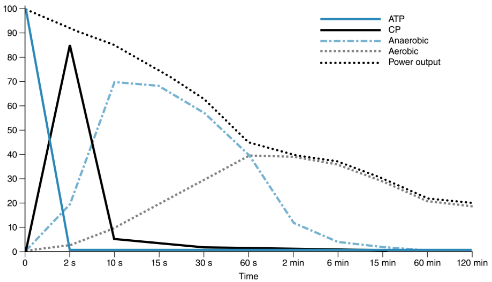
\includegraphics[scale=0.5]{visualisation/energy_provision.png}
    \caption{Energy provision by time \cite{Bompa.2018}}
    \label{fig:energy_provision}
\end{figure}
In general, a single training session can be split into multiple phases. During and shortly after the training session, the athlete is fatigued. After the training session has ended, the recovery starts. Recovery includes restoring energy stores in the muscles and reduce the lactic acid in the blood circulation. After many training sessions, the athlete's body starts to adapt to the constant exertion, i.e. the energy stores in the muscles increase or the heart muscle becomes stronger. This adaption process leads to improvement of the athlete's performance \cite{Bompa.2018.adaption}. Figure \ref{fig:training_improvement} visualises this adaption effect. The blue curve shows the performance of the athlete. With every stimulus, i.e. training session, the performance reduces to a minimum due to fatigue. After recovery, the maximum performance increases due to adaption.
\begin{figure}[ht]
    \centering
    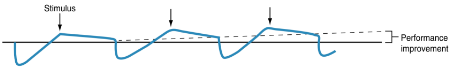
\includegraphics[scale=0.5]{visualisation/training_improvement.png}
    \caption{Performance improvement by continuous training \cite{Bompa.2018.compensation}}
    \label{fig:training_improvement}
\end{figure}
\subsection{Critical power concept} \label{critical_power}
In sports theory, critical power is the maximum rate that can be sustained for a very long time without fatigue \cite{Monod.1965,Hill.1993}. \citet{Monod.1965} introduced this concept and showed in their study that muscle power output and time to exhaustion follows a hyperbolic relationship while the total work performed is linearly connected to the time to exhaustion. Therefore, the critical power can be used as an indicator of the athlete's endurance and anaerobic capacity. With this indicator, coaches can optimise their training by setting loads and intensity in the aerobic area and evaluating the athlete's anaerobic performance without employing expensive material \cite{Dekerle.2002}. Other studies have shown that these concepts are applicable for swimming in general \cite{Wakayoshi.1992} and also for junior swimmers \cite{Hill.1995}. The critical power concept is of interest for our work as it gives us an idea of how the distances and the corresponding times are related.
\subsection{Machine learning for swim result prediction}
To the best of our knowledge, there is no related work that uses the same approach as we propose. However, some papers use similar data representation or try to achieve the same result but based on a different setting.\\
\citet{Silva.2007} use neural nets to predict the swimmer’s performance in 200m individual medley and 400m freestyle based on how the swimmer performs in multiple fitness, strength and flexibility tests. The authors submitted 138 junior swimmers of national level to four test categories: kinanthropometric, general functional and specific functional tests as well as an evaluation of their swimming technique. With the results of these tests, they predict the swimmer’s competition performance using Artificial neural nets. Moreover, they determine the physical factors that affect this performance the most. Although the ground truth, i.e. the data the model uses for training, is different from our, the machine learning approach itself is similar to our approach: They train a multilayer perceptron with one hidden layer and mean-squared error as loss function. \citet{EdelmannNusser.2002} use this machine learning approach as well. However, they try to predict the Olympic 200m backstroke performance of only a single swimmer. Therefore, their training data contains specific knowledge about the amount and intensity of training in the weeks before the respective competition. With this approach, they were able to predict the performance with a mean-absolute error of $\pm 0.62s$.\\
In order to predict how junior swimmers perform when they are older,, \citet{Xie.2015} divide 12- and 13-year-old top swimmers from the US into four performance level: the top 25\%, 25\%-50\%, 50\%-75\% and the last 25\%. A swimmer is represented by a single record of \texttt{(stroke, course, age, time, powerpoint)} where the powerpoint is a score that relates the swimmer's performance to other performances in this age group. Using SVM and neural networks, they determine the level change rate that is the probability that the swimmer will (still) be in the top-level when he is 18 years old. 
%\begin{itemize}
%	\item Lead up to your contributions.
%	\item Describe your research process.
%	\item Start with theoretical work and work yourself to its applications in your reproach report.
%	\item Document your implementation and solution to the problem described in previous sections.
%	\item Discuss your data collection, training or implementation approach and highlight interesting technical details.
%	\item Feel free to add more sections or subsections and rename existing sections e.g. the Contributions section as you need.
%\end{itemize}
\section{Design and implementation}\label{sec:contribution}
 




\section{Results \& Discussion}\label{sec:results}

%\begin{itemize}
%	\item Describe your results in a clrear and understandable way.
%	\item Clearly differentiate between what you have achieved and what you have build upon.
%	\item Ideally add some sort of visual representation of your result that underlines the progress you have made during the research project.
%	\item Make sure that the results are reproducible by your reader if needed
%	\item Critically discuss your results.
%	\item Did you achieve what you set out to do?
%	\item What are the strengths and weaknesses of your research?
%\end{itemize}
In this section, we discuss our dataset, evaluate our machine learning model and present our final mobile application.
\subsection{Dataset}


\subsection{Android application}

\section{Future Work \& Conclusion}

%\begin{itemize}
%	\item Summarize your thoughts and state your final conclusion about the work you have performed.
%	\item Describe possible future work in the field that is related to you work.
%	\item Detail improvements that could be done to your work in a following project.
%	\item Identify the importance of your work and create an arch to the related work and problem defined in the previous chapters.
%\end{itemize}
In this paper, we introduced an appealing application that helps coaches to estimate their swimmers' performances. However, the underlying machine learning model does not achieve the results we hoped. One reason for this is that we focus on non-professional swimmers; thus, their performance is less constant and therefore, less predictable. Nevertheless, the coaches of these swimmers need the most assistance; thus, a reliable prediction model is of high interest. A possible improvement could be to include more data, especially for the slower 50m times to find a correlation in our data, or use data augmentation to generate more samples from the existing data.\\
Another problem is that the swimmer's performance changes within a season. In our approach, we use an age representation based on the age group of the swimmer instead of his actual age. Therefore, it would be better to include the swimmer's age in month and, more importantly, the information at which point in the season the competition took place.\\
As the related work suggests, the swimmer's anthropometry is of high importance for his performance. Therefore, it would be good to include the height or flexibility in our records. We are currently working on a different approach that includes information about the training status of the swimmer. Therefore, we collect data about the four weeks before the respective competition. This data includes the total amount of training in kilometres as well as the intensity of the training sessions, i.e. the amount of training in the aerobic area or the number of technique sessions. The first results are already promising. However, for this approach, it is indispensable to work together with a group of swimmers as the needed data is not publicly available. \\
To get a first evaluation of our approach, we had to make some constraints. If we find a good data representation to predict results, we can enlarge our predictions to different strokes and distances, as well as include times swam in a 50m pool.
\FloatBarrier
\bibliographystyle{IEEEtranN}
\bibliography{references}

\end{document}
